%% This LaTeX-file was created by Marco Kienzle (Marco.Kienzle@gmail.com)
%% 
%% Do not edit this file unless you know what you are doing.

\documentclass{article}

% Language & comments
%\usepackage[french, english, swedish]{babel}	

\usepackage{amsmath}
\usepackage{amssymb}        % pi, infinity, natural/real symbol...
%\usepackage{hyperref} 		% interactive pdfs 
%\usepackage{apacite}        % APA
\usepackage[comma]{natbib}	  % citation
\usepackage{pdfpages}


%\usepackage[dvips]{color}

%\usepackage{natbib}
\usepackage{authblk}
\usepackage{setspace}
\usepackage{amsmath}
\usepackage{graphicx}
\usepackage{etoolbox}
\makeatletter
\patchcmd{\Ginclude@eps}{"#1"}{#1}{}{}
\makeatother
%\usepackage{psfig}
\usepackage{verbatim}
\usepackage{rotating}
\usepackage{multirow}
\usepackage{longtable}
\usepackage{booktabs}
\usepackage{subfigure}
\usepackage{lineno}
\usepackage{pbox} % multiple line in table cells
\usepackage{url}

\usepackage{fancyhdr}
\pagestyle{fancyplain} %Note the \fancyplain command !!!
\fancyheadoffset{1 cm} 
%\renewcommand{\chaptermark}[1]{\markboth{#1}{}}
%\renewcommand{\sectionmark}[1]{\markright{#1}{}}
\lhead[\fancyplain{E}{EE}] {\fancyplain{}{}}
\chead[\fancyhead{}{}]{\fancyplain{}{Draft}}
\cfoot [ ] {\copyright \hspace{0.1cm} State of Queensland through the Department of Agriculture and Fisheries (2017) \begin{center} \thepage \end{center}}

\setlength{\oddsidemargin}{0.5cm}
\setlength{\evensidemargin}{0.5cm}
\setlength{\textwidth}{17cm}
\renewcommand{\baselinestretch}{2.0} % set space between lines to 1.5
\DeclareMathOperator*{\argmax}{arg\,max}

\begin{document}
\linenumbers

%\title{Optimal harvest strategy for fishing tiger prawns in Moreton Bay according to a Markov Decision Process}
%\title{Optimal Economic Harvest Strategy from a Markov Decision Process applied to a delay-difference model: insights from the tiger prawn fishery in Moreton Bay (Australia) case study}
\title{Optimal Harvest Strategies according to a Markov Decision Process applied to a delay-difference model: insights from the tiger prawn fishery in Moreton Bay (Australia)}
\author[1,2,5]{Marco Kienzle}
\author[3,4]{Martin P\'{e}ron}
\author[3]{Sam Nicol}
\author[3]{Yann Dujardin}
\author[3]{Iadine Chad\`{e}s}

\affil[1]{Queensland Department of Agriculture and Fisheries, Dutton Park QLD 4102, Australia}
\affil[2]{Centre for Applications in Natural Resource Mathematics, School of Mathematics and Physics, University of Queensland, Australia}
\affil[3]{CSIRO, GPO Box 2583, Brisbane QLD 4001, Australia}
\affil[4]{School of Mathematical Sciences, Queensland University of Technology, Brisbane QLD 4000, Australia}
%\affil[5]{Somewhere in Europe}
\affil[5]{Corresponding author: Marco.Kienzle@daf.qld.gov.au}

\maketitle

%\tableofcontents
\clearpage
\newpage

\abstract{A Markov Decision Process (MDP) is a mathematical framework, developed in the 1950s, to optimise sequential decisions in a probabilistic model. Today, it is applied in a wide range of industries but seldom to manage fisheries despite its relevance to the governance of marine resources. In this paper, we applied a MDP to a delay-difference model calibrated to capture the dynamics of a trawl fishery targeting tiger prawn ({\it Penaeus esculentus}) in Moreton Bay, Australia. This bio-economic model of the fishery explored harvest control rules that maximized the economic profit of the fleet in response to variable economic and environmental conditions. Accounting for these uncertainties, a MDP suggests that the industry is operating at or its near optimal level given the regulatory and environmental constraints on the fishery. It shows that the Maximum Economic Yield (MEY) is achieved by adapting effort in response to abundance and economic conditions, notably by increasing fishing effort when the resource is more abundant. This MDP application to a tiger prawn fishery concludes that economic conditions and regulatory measures currently in place are constraining fishing effort well below the levels of effort that produce the Maximum Average Yield (MAY) or Maximum Sustainable Yield (MSY). Hence this stock is not currently at risk of becoming over-exploited. Simulations comparing the optimal strategy to other fishing strategies showed that (a) fishing the stock every year at MAY is un-profitable in the prevailing economic conditions, performing even worse than a random level of effort and (b) fishing every year at levels of effort 60\% lower (4,000--5,000 boat-days) than the maximum effort recommended by a MDP (7,000--8,000 boat-days) returns profits 89\% smaller than the optimal policy. By applying an MDP to this fishery, we contrast the notion of a static reference point (MSY and MEY) to the notion of dynamic changes in effort in response to stock abundance. The MDP policy yields greater profits than the other strategies due to its ability to adapt fishing effort in response to changing environmental and economic conditions.}
\section*{keywords}
Markov Decision Process, bio-economic model, delay-difference model, brown tiger prawn

\clearpage
\newpage

\section{Introduction} In fisheries, a harvest strategy is a rule to adjust fishing intensity in response to the abundance of an exploited natural resource to meet sustainability and economic or social objectives \citep{hil92b}. A harvest strategy is not a set of annual regulations; it has to be robust to unpredictable biological fluctuations affecting a stock. The productivity of short-lived species such as prawns is determined by the strength of recruitment each year and most effectively managed by effort control \citep{garcia88c}. There is a need to provide harvest strategies that balance the sustainability of fisheries with industry profitability. This problem is inherently stochastic because recruitment varies from year to year in response to environmental and fishing factors \citep{KienzleEtAl2017}. Deterministic approaches fail to account for the natural variability affecting such systems, leading to harvest rules inflexible to changes in recruitment. Markov Decision Processes (MDP) can address this problem elegantly because they provide a framework for decision-making in uncertain situations \citep{puterman_markov_1994}. This method accounts for the relationship between present and future decisions and provides an optimal state-dependent management strategy to the problem: an optimal policy. There have been a handful of MDP applications in fisheries research focusing on the number of fish left to spawn \citep{Mendelssohn1980a, LUDWIG1982273} which suggested that maintaining a constant escapement strategy was the optimal harvest strategy. These results have proved to be more of a hindrance than a help in designing good harvest strategies \citep{hil92b} because maintaining a constant stock-size is difficult to achieve in a naturally variable world and measuring stock abundance, before or after fishing, is challenging. The last decade has seen an explosion of successful usage of MDPs in artificial intelligence, providing a robust approach for autonomous systems to learn from and adapt to their environment by interacting with it \citep{Kochenderfer:2015:DMU:2815660}. Similarly, in the the field of species conservation there has been an increase in MDP usage, with applications in biological invasions \citep{firn_managing_2008,regan_optimal_2006}, disease management \citep{chades_general_2011}, release of biocontrol agents \citep{shea_optimal_2000}, harvesting \citep{williams_adaptive_1996}, migratory species \citep{nicol_adaptive_2013}, recovery of interacting species \citep{chades_setting_2012} and fire management regimes \citep{mccarthy_using_2001,possingham_optimal_1997,richards_optimal_1999}. \\

Moreton Bay is a large estuary-fed bay in Queensland situated near the southern limit of the distribution of tiger prawn ({\it Penaeus esculentus}) on the east coast of Australia (Fig.~\ref{fig:Map}). In this area, the stock of tiger prawns is managed by input control through gear restriction (fishing license, vessel size limited to up to 14m in length, net head-rope length) and temporal and spatial area closures to avoid conflicts with recreational users \citep{Pascoe2017121}. Currently, effort is capped in this fishery at a maximum of 32,100 boat-days, however not more than 4,900 days have been used in Moreton Bay since 2008. Contrary to other fisheries in Australia ({\it e.g.} \cite{Dichmont05012010}), the total amount of effort targeted at tiger prawn each year is not controlled by fisheries managers but by fishers who assess the abundance of new recruits on the fishing ground at the beginning of each fishing season to determine if and when it becomes economical to target tiger prawns (Moreton Bay Seafood Industry Association pers. comm.) effectively adapting their response to economic factors and the relative species abundance. The size of the fishing fleet has decreased by 60\% in the last 20 years as a result of increasing competition in the seafood market from other prawn fisheries, aquaculture production and increasing costs of fishing such as rising fuel prices \citep{Pascoe2017121, FAO2016}. Tiger prawn exploitation in Moreton Bay is assessed as being sustainable according to a single species delay-difference model which estimates all parameters to describe the dynamics of this fishery including recruitment \citep{KienzleEtAl2015, Kienzle2014138}. Maximum Sustainable Yield (MSY) or Maximum Average Yield (MAY\footnote{MSY and MAY are used interchangeably in this text. MAY was defined by \cite{Mace2000MSYa} as '... most fisheries scientists now interpret MSY in a more dynamic sense as the maximum average yield (MAY) obtained by applying a specific harvesting strategy to a fluctuating resource.'}) was estimated at 200 $\pm$ 50 tons per year, similar to that estimated by a multi-species model of this fishery \citep{NaWang2015a}. The largest uncertainty about the dynamics of this stock is recruitment, estimated with a delay-difference model, which fluctuates between years: the best predictor of recruitment estimated with a delay-difference model \citep{KienzleEtAl2015} found to date is water temperature which explains 69\% of its variability \citep{KienzleEtAl2017}. \\

The stock of tiger prawns in Moreton Bay does not have a harvest control rule (HCR). Although the exploitation of tiger prawn in Moreton Bay is sustainable at present, developing a harvest control rule may provide fisheries managers with insights into how and why fishers make decisions about when to fish, and aid managers to better understand and work with fishers to ensure that the stock remains sustainable without over-regulating the fishery. We applied a MDP to define a harvest control rule that maximizes the profit of the fishing industry while maintaining the capacity of the stock to withstand exploitation and regenerate itself year after year. Bio-economical models have been used previously to assess tiger prawn fisheries and the federal government of Australia has a history of using economic target reference points to manage some of its commercial fisheries \citep{Kompas2010a}. Previous analyses have ignored the effect of future recruitment variability on management advice because of the computational demands of bio-economic analyses (e.g. \cite{punt2010a}). The mathematical formulation of a MDP overcomes the computational problem and allows for the inclusion of the full spectrum of uncertainties. In particular, MDP overcomes the uncertainty about the magnitude of recruitment given the spawning stock size and can compute the optimal harvest control rule efficiently. Our MDP approach provides a Maximum Economic Yield (MEY) policy which defines optimal effort in response to the abundance of stock each year, accounting for the effect of fishing in the previous year, biological uncertainty in stock productivity as well as cost and revenue from fishing. We used this bio-economic model to investigate how different costs and revenue influence optimal levels of fishing effort, sustainability and economic profitability of the fishing fleet to provide a harvest control rule that achieves maximum economic yield while preserving the ability of the stock to regenerate itself. This analysis focused on a single species, the tiger prawn ({\it Penaeus esculentus}), because population dynamics models for other species caught by trawlers in this area have not been developed. Twenty-one years of catch and effort data recorded since 1990 have been used to identify the optimal harvest strategy presented in this document. This analysis was developed to account for the biological traits of the species, the characteristics of the fleet and environmental fluctuations affecting catch and recruitment \citep{KienzleEtAl2015}. It provides a fishing policy that maximizes surplus production and profitability of the fleet.\\



\section{Materials and methods} 
%\documentclass[10pt]{article}

% Language & comments
%\usepackage[french, english, swedish]{babel}	

%\usepackage{amsmath}
%\usepackage{amssymb}        % pi, infinity, natural/real symbol...
%\usepackage{hyperref} 		% interactive pdfs 
%%\usepackage{apacite}        % APA
%\usepackage[comma]{natbib}	  % citation
%\usepackage{pdfpages}
%\DeclareMathOperator*{\argmax}{arg\,max}

%\begin{document}
%\selectlanguage{english}

%\section{Materials and Methods}

%We start by formally introducing Markov decision processes and stochastic dynamic programming.\\

\subsection{Markov decision processes}

Markov decision processes (MDP) are mathematical frameworks for modelling sequential decision problems where the outcome is partly stochastic and partly controlled by a decision-maker \citep{bellman_dynamic_1957}. A MDP is defined by five components $< S, A, P, r, C >$ \citep{puterman_markov_1994} : (i) a state space $S$, (ii) an action space $A$, (iii) a transition function $P$, (iv) an immediate rewards function $r$ and (v) a performance criterion $C$ (Fig.~\ref{fig:mdp}). In our system, the state space represents the amount of prawns recruiting to the fishery each year and the action space the total amount of fishing effort applied each year. The transition function captures the impact of fishing on future states of the stock.

The decision-maker aims to direct the process towards rewarding states. From a given state $s$, the decision-maker selects an action $a$ and receives a reward $r(s,a)$. At the next time-step, the system transitions to a future state $s'$ with probability $P(s'|s,a)$\footnote{$P(.|.,a)$ is a transition matrix, {\it i.e.} each row is a probability distribution over future states $s'$.}. The performance criterion $C$ specifies the objective, the time horizon (finite or infinite), the initial state $s_0$ and whether there is a discount rate ($\gamma$). Here, our objective is to maximize the discounted sum of expected ($\mathbb{E}$) rewards over an infinite time horizon: 
\begin{equation}
\mathbb{E}[\sum\limits_{t=0}^\infty \gamma^t r(s_t,a_t)|s_0]
\end{equation}

A policy $\pi$ describes which decisions are made in each state, i.e. $ \pi : S \rightarrow A$. Solving a MDP means finding an optimal policy $\pi^*$, which satisfies in our case:
\begin{equation}
\pi^* = \argmax_\pi \mathbb{E}[\sum\limits_{t=0}^\infty \gamma^t r(s_t,\pi(s_t))|s_0]
\end{equation}

Methods to solve MDPs can be classified into linear programming, value iteration and policy iteration \citep{sigaud_markov_2010}. We choose to use policy iteration, for its efficiency \citep{sigaud_markov_2010} and simplicity. Interested readers can refer to supplementary information for details about the policy iteration algorithm (supplemental materials, section~\ref{SuppSection-PolicyIterationAlgo} p.~\pageref{SuppSection-PolicyIterationAlgo}). We computed solutions to this problem using the MDPtoolbox package in R \citep{MDPtoolbox}.




\subsection{From calibrated stock assessment model to transition matrix}

%\paragraph{Parameterizing the MDP using the stock assessment model} \mbox{} \\

% a weekly delay difference was used to represent the dynamic of this stock in response to environmental and fishing pressure.
% Calibration the model
% Stock-recruitment relationship
% Simulated dataset. Calculating MSY ( = 209 +- 79 tonnes) for 20500 boat-days of effort.

A delay-difference model, calibrated to logbook data \citep{KienzleEtAl2015}, was used to generate synthetic data about the tiger prawn fishery in Moreton Bay. Those data were converted into a transition matrix required as an input to the MDP method.

\paragraph{Tiger prawn stock assessment model}

This weekly biomass ($B_{w}$) dynamic model of brown tiger prawn consists of a delay-difference model \citep{sch85a} fitted to logbook data collected between 1990 and 2010 and grouped into weekly timesteps: 

\begin{equation}
B_{w} = s_{w-1} \ B_{w-1} + \rho \ s_{w-1} \ B_{w-1} - \rho \ s_{w-1} \ s_{w-2} \ B_{w-2} - s_{w-1} \ \rho \ w_{k-1} \ R_{w-1} + w_{k} \ R_{w} \ ,\  3 \leq w \leq 1092
\end{equation}

Sex-combined growth parameters ($\rho$ = 0.963, $w_{k-1}$ = 17.8 g and $w_{k}$ = 19.5 g), derived from von Bertalanffy estimates \citep{grib94a}, were fixed in the model. This model assumed all prawns were fully recruited to the fishery (knife-edged selectivity) at an age of 22 weeks ($k=22$), weighing 19.5 grams. Survival ($s_{w}$) varied as a function of natural mortality rate ($M$) and fishing mortality ($F_{w}$) which is proportional to effort ($F_{w} = q E_{w}$). Natural mortality ($M$), catchability ($q$) and recruitment ($R_{w}$) were estimated by fitting the delay-difference model to logbooks data \citep{KienzleEtAl2015}. This model included all environmental and fishing effects known to influence the dynamics of this population of prawns: temperature has been recognized as a factor influencing availability of prawns and the effect of fishing accounts for both changes in fishing power through time as well as catchability \citep{KienzleEtAl2015}.

\paragraph{Calibrating the stock assessment model}

A total of 29 parameters (two catchability parameters, two initial biomass ($B_{1}$ and $B_{2}$), two von Mises parameters, one natural mortality, twenty one annual recruitment parameters and $\sigma$, one standard deviation of observation errors) were estimated by maximum likelihood assuming the square-root of predicted catch ($\hat{C}_{w}$, \cite{quin99b}) 

\begin{equation}
        \hat{C}_{w} = \frac{q \ E_{w}}{ M + q \ E_{w}}  B_{w} ( 1 - \exp[-(M + q \ E_{w})])
\end{equation}

\noindent provided the mean of a Normal distribution of the square-root of observed catches ($C_{w}$) \citep{dichmont2003application} with residual standard deviation ($\sigma$). The negative log-likelihood function used to fit the model was \citep{haddon2010modelling}

\begin{equation}
-\log(L) = n \ log(\sqrt{2 \pi} \sigma) + \frac{1}{2 \sigma^{2}} \sum_{w=1}^{1092} \bigl ( \sqrt{\hat{C}_{w}} - \sqrt{C_{w}} \ \bigr ) ^{2}
\end{equation}

The model was implemented in C++ and used the MINUIT minimization library \citep{minuit2} available through ROOT \citep{root}. The code of this delay-difference stock assessment model is available at \url{https://github.com/mkienzle/DelayDifference}.

\paragraph{Closing the life-cycle with a recruitment model} 
Investigations of a relationship between spawning stock biomass and recruitment found fitting Ricker stock-recruitment relationship (SRR) was not significant \citep{Kienzle2014138}. Beverton and Holt SRR provided a better fit to the data \citep{KienzleEtAl2017} and was used to relate the abundance in successive generations of prawns:

\begin{equation}
    \begin{split}
  &{\rm log} \Bigl(\frac{R_{t}}{S_{t}}\Bigr) = 16.1 - {\rm log}(972.5 + S_{t}) + \varepsilon_{t} \\
  &\varepsilon_{t} \sim \mathcal{N}(\mu=0,\,\sigma^{2}=0.4)  
    \end{split}
  \end{equation}

\noindent Where $R_{t}$ is the total number of recruits each year and $S_{t}$ is the spawning stock biomass (SSB) in kg. The random noise masks most of the signal from the SRR (Fig.~\ref{fig:BevertonAndHoltSRR-NaturalScale-WithCategories}) resulting in recruitment levels that are random for almost all levels of SSB except for the lowest. Total number of recruits each year ($R_{t}$) were distributed weekly in the simulations using a von Mises distribution \citep{mardia1999directional} with mean and concentration parameters set respectively to 0.53 and 4.74.

\paragraph{Biological reference point} We calcualted Maximum Sustainable Yield (MSY) or Maximum Average Yield \citep{Mace2000MSYa} by simulation using SRR in combination with the calibrated delay-difference model over periods of 50 years. We performed 310,000 replications with effort ranging from 0 to 30,000 boat-days per year to plot the distribution of catch in the final year as a function of effort (Fig.~\ref{fig:ProjectedCatchvsEffort}). Total simulated yearly effort was distributed among the 52 weekly time steps, used in the delay-difference model, applying the average pattern of fishing targeted at tiger prawn \citep{Kienzle2014138}) observed over the last 5 years of data (2006--2010) (Fig.~\ref{fig:EffortPattern}). Maximum Average Yield (MAY) was estimated to equal 217 $\pm$ 85 tonnes, similar to those estimated by \cite{NaWang2015a}, and larger than the 145 $\pm$ 53 tonnes obtained with Ricker's SRR \citep{Kienzle2014138}: replacing the dome-shaped Ricker by an asymptotic Beverton-Holt's SRR had a significant effect on the estimation of effort at MAY ($\rm{E_{MAY}}$), increasing it 4 fold to 19,500 compared with 5,400 boat-days estimate in \cite{Kienzle2014138} and 5157 boat-days, ranging from 3531 and 7912 boat-days, estimate in \cite{NaWang2015a}. Such high uncertainties about reference points are common in fisheries research \citep{hil92b}.

\paragraph{Transition matrix} We chose recruitment as the state variable and fishing effort as the action of the MDP. We computed the transition matrix from simulated data generated as described above. We varied total yearly effort ($E_{t}$) between 0 and 30,000 boat-days, drawing for each simulation uniformly within the following 31 categories 0, [1;1,000), [1,000; 2,000), ..., [29,000; 30,000] and distributed into 52 weekly effort values ($E_{w}$) using the pattern of weekly effort observed in the fishery between 2006 and 2010 (Fig.~\ref{fig:EffortPattern}). We replicated simulations over a 50-year period 10,000 times for each effort category to create a set of simulated data. We used recruitment in the last 2 years of the 50-year simulations to compute the transition between recruitment in year $t$ and $t+1$ to reduce the influence of initial simulation conditions. We binned simulated recruitment into three categories bounded by the 0\%, 33\%, 66\% and 100\% percentiles of its distribution, representing 3 categories of tiger prawn recruitment (low, medium and high). These categories correspond to the following ranges of number of recruits: [1.19e+06; 7.81e+06), [7.81e+06; 1.12e+07) and [1.12e+07; 6.62e+07]. As a result, we obtained a three-dimensional transition matrix, of size $(S,S,A)$= (3,3,31), representing the probabilities for the stock of tiger prawn transitioning from a particular state of recruitment (low, medium and high) in year $t$ to any category of recruitment in year $t+1$ after being fished with fishing effort belonging to one of the 31 categories of fishing effort. (Fig.~\ref{fig:BubblePlotOfTransitionMatrix}).\\

The state variable in a MDP must have the property of a Markov process. We assessed this property using an analysis of auto-correlation applied to the simulated recruitment time-series, lagged between 1 and 10 years, using the auto-correlation function (acf) available from the R-package MASS \citep{MASS}. This analysis showed simulated recruitment to be auto-correlated significantly only for a lag of 1 year ($\rho=2.25e-02$, ${\rm P-value} < 2.2e-16$) confirming that it has the property of a Markov process.

\paragraph{Economic model} The reward from the action ($a$) of fishing each year with level of effort ($E_{t}$) was rewarded ($r(s,a=E_{t})$) by the profit, in dollars (\$), calculated as the difference between revenue (i.e. catch per year ($C(s,a)$ in kg) times the price per kg of prawns ($P$)) minus the cost of fishing (i.e. effort ($E_{t}$) times cost per unit effort ($\xi$ in \$ per boat-day)), for the entire fleet each year:

\begin{equation}
r(s,a=E_{t}) = C(s,a=E_{t}) \ P - \xi \ E_{t}
\end{equation}

This choice was made after investigating both catch and catch per unit effort as reward functions and noticing that they provided unrealistic and unobserved optimal strategies. \\
The yearly catch was calculated with the weekly delay-difference model: $C(s,a=E_{t})=\sum_{w=1}^{52} \hat{C}_{w} $ where $E_{t} = \sum_{w=1}^{52} E_{w}$. 

The price of prawns per kg ($P$) was varied between \$6 and \$40; the cost of fishing was varied from \$0 to \$500 by \$100 increments.\\

%Previous bioeconomic analyses of similar prawn fisheries showed MEY to be more sensitive to price of prawns and fishing costs changes than discount rate values \citep{Kompas2010a}. The discount rate was set to $\gamma=0.9$.
The discount factor ($\gamma$) is a parameter in the MDP which captures the value of money to fishers at a given time relative to its value one time step earlier: a small $\gamma$ favors making money by fishing in the present while a value close to one puts almost equal weight to money made in the present or into the future. The profit function in the MDP measures the income made by fishers from catching tiger prawns. The necessity for fishers to make an income every year situates the value of $\gamma$ probably above and beyond inflation (2.5\% per year) and interest rates (4.5\%/yr) combined corresponding to $\gamma < 0.93$. Nevertheless given the uncertainty on this parameter, we performed the analysis with $\gamma$ ranging from 0.6 to 0.98. 

\section{Results} State transition matrices which provide the probability that recruitment changes from low, medium or high level from year $t$ to year $t+1$ were calculated with the fishery model using 31 possible fishing intensities (Fig.~\ref{fig:BubblePlotOfTransitionMatrix}) ranging from 0 to 30,000 boat-days. The transition matrix when no fishing occurs (top-left in Fig.~\ref{fig:BubblePlotOfTransitionMatrix}) shows that recruitment at time $t$ has nearly equal probability ($0.31 \leq P(s_{t+1}|a_{1}, s_{t}) \leq 0.37$) to be followed by any magnitude of recruitment at time $t+1$ with a slightly larger chance (37\%) of a low level of recruitment being followed by a high level of recruitment than a low level of recruitment (31\%). At the other extreme of the spectrum of actions, where fishing effort used in the simulations is within the largest category considered in the simulations (29,000--30,000 boat-days), the recruitment is more likely to be low at time $t+1$ irrespective of recruitment at time $t$; the probability of a high recruitment following a low recruitment (24\%) is the smallest of all future states while the probability of a low recruitment being followed by a low recruitment is the largest (43\%). Intermediate levels of fishing effort, between 1,000 and 29,000 boat-days, resulted in transitions matrices intermediate to the two extreme cases described above. For example fishing with 19,000--20,000 boat-days, corresponding to effort level at MSY or MAY (E$_{\rm MAY}$): any level of recruitment in one year is equally probable to be followed by any level of recruitment a year after ($0.32 \leq P(s_{t+1}|a_{21}, s_{t}) \leq 0.35$). \\ %The choice of categories breaks to bin simulations results affected the results of the MDP because it influences these patterns in the transitions matrices. \\

The MDP showed that fishing strategies maximizing profit, for cases with cost of fishing $>$ \$0 per boat-day, were almost insensitive to the discount factor ($\gamma$): for $\gamma$ between 0.6 and 0.98, profit from exploiting tiger prawns in Moreton Bay is maximized by increasing effort as recruitment increases (Fig.~\ref{fig:SensitivityToDiscountFactor}). 
By contrast, the optimal policies obtained by maximizing catch, {\it i.e.} setting fishing costs to \$0 per boat-day, were more sensitive to the discount factor: at medium recruitment level, optimal efforts increased as the emphasis on catching fish in the present increased ($\gamma$ decreased). In the extreme case of valuing the present 1,000 times more than the future, $\gamma = 0.001$ (not shown in Fig.~\ref{fig:SensitivityToDiscountFactor}), the optimal strategy obtained was logically to fish at the highest level of effort possible for any level of recruitment. In the remainder of this section, the MDP solutions presented were computed for $\gamma = 0.8$ without loss of generality.\\

The method to calculate MAY estimated the maximum average catch over all possible levels of recruitment to equal to 217 $\pm$ 85 tonnes could be achieved with 19,500 boat-days of fishing effort per year (Fig.~\ref{fig:ProjectedCatchvsEffort}). This figure shows that $\rm{E_{MAY}}$ is extrapolated far removed from observed values. Increasing boat-days by a factor of four or more would have major impacts on the abundance of tiger prawns and other species caught by trawlers in Moreton Bay, in particular juvenile eastern king prawns. So rather than being proposed levels of fishing effort, these values are illustrative of what would be required to actually achieve MAY or MSY. Obviously, the economics of this fishery determine actual fishing effort, as follows.
%well beyond all levels of fishing effort observed between 1990 and 2010 in this fishery: it should be carefully considered for management purposes. Nevertheless, this estimate of $\rm{E_{MAY}}$ is consistent with the equivalent reference point calculated with the MDP: the MDP shows that maximum catch (Fig.~\ref{fig:SensitivityToDiscountFactor}, $\gamma=0.8$ and \$0 fishing costs) is achieved at low recruitment using 18,500 boat-days; at 19,500 boat-days at medium level of recruitment and at at 29,500 boat-days at high levels of recruitment. Contrary to the static nature of the calculations to estimate MAY, the MDP suggests that the best strategy to maximize tiger prawn catch is to apply more fishing effort in years of high recruitment rather than applying constant fishing effort ($\rm{E_{MAY}}$) irrespective of the fluctuations in recruitment. This dynamic interpretation of MSY indicated that such strategy yields 1 tonne more, none and 15 t more at low, medium and high levels of recruitment, respectively. \\

The MDP shows that including a profit function into the model with fishing costs of \$100 or more per boat-day is enough to constrain fishing effort below ${\rm E_{MAY}}$ (Fig.~\ref{fig:SensitivityToDiscountFactor}). The larger the costs, the smaller the fishing effort because profitable fishing is achievable only at higher abundance levels. The strategy that maximizes profit or Maximum Economic Yield (MEY) over an infinite number of years is to adapt effort in response to tiger prawn abundance and prevailing economic conditions. For example, the MDP shows that a low recruitment combined with high fishing costs (equal or above \$300 per boat-day) leads to no fishing on this species (Fig.~\ref{fig:SensitivityToDiscountFactor}, $\gamma=0.8$) due to negative profits when fishing occurs. 

The logbook data provide evidence that the fishing fleet, as a whole, has been behaving in agreement with the optimal strategy suggested by the MDP. First, the MDP suggested the industry should increase fishing effort when tiger prawn abundance is high to maximize profit: logbook data showed a statistically significant relationship (p-value=0.017) between effort and recruitment, explaining 23\% of the variability in effort (Fig.~\ref{fig:PlotEffortAgainstRecruitment})). Second, observed fishing effort and catches overlayed with the optimal MDP's policies (Fig.~\ref{fig:MDPonProfit-OverlayedWithObs} and ~\ref{fig:MDPonProfit-RecCatAgainstCatch-OverlayedWithObs}) suggested fishing effort deployed in Moreton Bay in response to tiger prawn abundance is consistent with optimal fishing strategies for costs of fishing varying between \$100 and \$400 per boat-day, with 80\% of observations falling between \$200 and \$300: the bio-economic models provide a more realistic description of the variation of effort in this fishery compared to the biological model that ignores economic factors and average catch across all recruitment variability to compute MAY. The average fishing effort catching tiger prawn between 1990 and 2010 is approximately 24\% of ${\rm E_{MAY}}$ (Fig.~\ref{fig:ProjectedCatchvsEffort}). Nevertheless, observed annual fishing effort appeared on average larger than predicted at low level of recruitment and smaller at high level: the observed variations of effort in response to abundance over time are not as steep as suggested by the MDP's optimal policies which assumed constant prawn prices and cost of fishing over the entire period. 

In comparison with traditional harvest strategies used in fisheries \citep{hil92b}, optimal strategies suggested by this MDP range from a constant escapement when cost of fishing is between \$300 and \$500 to proportional harvest when cost of fishing is \$0 or \$100 (Fig.~\ref{fig:MDPonProfit-RecCatAgainstCatch-OverlayedWithObs}). This suggests that economic factors do and can be used to alter fishing effort. Moreover, the economics of the fishery are constraining optimal fishing effort below $\rm{E_{MAY}}$ as illustrated by hypothetical scenarios varying prices of prawns from \$6 to \$40/kg (Fig.~\ref{fig:SensitivityToPrawnPrice}). Optimal fishing effort is positively correlated with profitability: a decline in prawn price by \$1 induces a decline in fishing effort by 300--500 boat-days per year; while increasing costs by \$1 per day of fishing reduces total effort by 20 boat-days a year. \\%A variation in prawn price by \$1/kg induces a variation in fishing effort of 500 boat-days per year.  \\

We used simulations to  compare the performance of the optimal strategy suggested by the MDP to alternative harvest strategies. Since this fishery does not have a HCR in place, we compared the outcome of applying an optimal strategy to that of applying (1) random effort; (2) constant low effort level (4,000--5,000 boat-days) and (3) constant effort at $\rm{E_{MAY}}$ (19,000--20,000 boat-days). These stochastic simulations, conducted over a 50 year period each, involved variable recruitment intensity and fishing effort varying or not according to the magnitude of recruitment (Fig.~\ref{fig:CompareVariousStrategies-1Simulation-TimeseriesOfStates} and ~\ref{fig:CompareVariousStrategies-1Simulation-TimeseriesOfActions}). The average yearly profit differed between strategies (Fig.~\ref{fig:CompareVariousStrategies-1Simulation-CumulativeReward}). A 1,000 replications of such simulations (Fig.~\ref{fig:CompareVariousStrategies-repeat1000times}) showed that constant effort at $\rm{E_{MAY}}$ and random effort strategies yielded negative profits in all simulations while the other two strategies were always profitable. The optimal strategy yielded the highest yearly profits, ranging from \$0.51 and \$0.87 million per year, with a median profit of \$0.70 million per year. The constant low effort strategy achieved profits ranging between \$0.45 and \$0.80 million per year, with a median profits of \$0.62 million (89\% of the optimal strategy). \\

% Comparison between optimal yield at constant (MSY) and variable fishing effort (MDP)

%Policies evaluations for a given price (12 \$/kg of prawn) and a range of costs of fishing, varying between 0 and 500 \$/boat-day, identified that the optimal fishing policy is to respond to a larger abundance by fishing more intensively (Fig.~\ref{fig:MDPonProfit}). \\
%The optimal strategy to maximize catch, given by maximizing the profit function fixing costs to zero, is to increase effort in response to larger abundance of the resource beyond fishing effort at MSY. This dynamic strategy achieves higher yields [ is is possible to calculate how much more catch than MSY ] and constrasts with the traditional, static,  view that Maximum Sustainable Yield is achieved at a fixed level of effort (show this on the graph).


%these discrepancies might arise from differences in optimal decision making between humans and algorithms induced by emotional responses such as the "sunken cost falacy".\\

%Varying fishing costs showed that when they are low, fishing can be profitable even at lower level of abundance.
%Varying fishing costs in the reward function showed that as they increase, there is a threshold abundance below which it becomes un-profitable to fish: the economics of fishing acts like a self protective mechanisms against biological over-fishing by stopping fishing at the lowest stock level. Varying both costs and prices of prawns showed that average fishing effort in the fishery declines as prawn prices decline and fishing cost increases (Fig.~\ref{fig:EffortSurface}). The total profit of the fishery is a declining function of cost of fishing at a given cost of fishing (Tab.~\ref{tab:AverageValueAsFctPricesAndCosts}) and an increasing function of price for a given cost. For example, at 12 \$/kg and 200 \$/boat-day, this stock will return an average profit of 5 M\$ per year. 




\section{Discussion} MDPs provide a well established and robust framework to compare various fishing strategies accounting for uncertainties in the system. The strength of this method is to embrace the dynamic nature of the fishery, and provide results that emphasize how adapting fishing effort to abundance maximizes profit. The range of effort maximizing profit was close to that estimated by a multispecies deterministic model reporting ${\rm E_{MEY}}$ ranging between 4.000 and 7.000 boat-days \citep{NaWang2015a}. The optimal harvest strategy is qualitatively and quantitatively in good agreement with changes in fishing effort observed in Moreton Bay over a 21-year period suggesting that fishers operate collectively at or close to the economic optimum. Larger observed annual fishing effort than suggested by the optimal harvest strategy at low level of recruitment might arise from differences in decision making between not so rational human behaviour and algorithms: the "sunken cost fallacy" as described in the field of behavioural economics has been widely observed in business ventures pursued beyond the point of economic rationality \citep{camerer2011advances}. The validity, realism and usefulness of the MDP results depend largely on the calibration of the delay-difference to logbook data as the MDP application itself is a deductive process based on the information encoded into the transitions matrix. \\

% devising an HCR based only on biological and ecological knowledge lead to policies that are inconsistent with the economic reality of the fishery, especially when the dynamics variation of abundance is not taken into account: caping effort at ${\rm E_{MAY}}$ leads to a target that is not reached a low levels of abundance because it is un-profitable and to loss of profits at high abundance. In other words, accounting for economics in designing policies provides a more adequate solutions to managing this and other fisheries.

% Good agreement between the data and the MDP results imply that the fishing fleet response to abundance and economics is very close to the optimal suggested by the MDP despite that fishing decisions were taken by each individual skipper and the model maximizes profit at the level of the fleet. 

The HCR that maximizes economic return to the industry while protecting the capacity of the tiger prawn stock to regenerate itself in Moreton Bay is to let effort, and catch, vary from year to year in response to unpredictable variations in stock size. Given recruitment of tiger prawns and stock size are the most uncertain aspects of the dynamics of this fishery, the best harvest strategy is neither to implement a total allowable catch \citep{Beddington1977} nor to impose season closures \citep{hil92b} but to allow fishers to adapt fishing effort to both biological and economical conditions. Managing prawn fisheries using effort instead of catch is made all the more important by their short-lived nature which makes abundance estimates very difficult \citep{parsons1993management}. The drawback of managing this fishery by input control is the resulting variability in catch potentially creating an over-supply of prawns and associated decline in prices. Nevertheless, the MDP policy presented here, which maximizes profit, has to be kept in perspective with the fact that only effort was allowed to vary in this study whereas more substantial increases in profit would have been achieved by also allowing catchability to increase. \\

%The economic model used is simple because the small size of the fishery precludes using complex (expensive) models.
% The economic model suggest increasing catch but does not take into account of the possible negative effect of larger catches on prawn prices.
The present implementation of the economic model, which is similar to that used in other bio-economic models ({\it e.g.} \cite{Dichmont05012010}), is simple in that it assumes fixed prices and costs over time. It is remarkable that despite its simplicity and the assumption that effort is adjusted by a single centralized entity maximizing its profit, the results are very similar to those observed from the sum of decisions made at the level of around 140 vessels over the period studied. This economic model was deliberately kept simple because the trawl fishery in Moreton Bay is too small to justify expensive data collection and analyses. As a consequence detailed economic information available to date is sporadic and imprecise preventing the development of more complex, dynamic, models. Had time series of prawn prices and fishing costs been collected over the last three decades, it would have been interesting to evaluate whether this simple economic model is capable of mimicking the declining fishing effort trajectory observed since 1990 perceived as resulting from the decline in prawn prices and increase in fuel costs over this period \citep{Pascoe2017121}. \\

This application of a MDP clearly demonstrates the influence of economical aspects of the fishery. Previous modelling work has evidenced that economic factors can increase fishing pressure on fish stocks in unregulated fisheries \citep{quin99b}. Instead, the present model of a regulated fishery suggests that economical factors and regulations act to limit the total effort expended in the fishery, preventing exploitation to become unsustainable. Further, effort levels required to achieve MAY appear unprofitable in the current economic and regulatory circumstances. This re-iterates the position long argued by some economists that a fishery maximizing its economic potential usually satisfies conservation objectives as well \citep{clark2017a}, at least in the low subsidy system characteristic of Australian fisheries. This position may be valid for Moreton Bay but not for the many fisheries in other jurisdictions that sustained perfectly economically viable businesses while increasing effort beyond ${\rm E_{MAY}}$ into a state of over-exploitation \citep{hilborn2011overfishing}.  \\

In practice, this work suggests that the tactics needed to implement the optimal harvest strategy each year have been performed successfully by the members of the fishing industry and the fishery management agency does not have to regulate effort in this fishery on a year-to-year basis as done for example in other prawn fisheries ({\it e.g.} \cite{Dichmont05012010}): it is not in fact the role of a harvest strategy \citep{hil92b}. Such tactical decisions are probably more efficiently made by fishers based on their knowledge of costs and landing prices specific to their own businesses. %rather than attempting to transfer this decision making process into an economic model of fisherman's behaviour that would be costly to develop, inflexible and difficult to maintain. Instead, this analysis suggests that the government agency responsible for managing this resource could play a more strategic role by developing policies that influence both side of the profit function in order to influence the exploitation of this resource. For example increasing revenue to attract new effort into this fishery, to develop the local economy and to increase profit from exploiting this resource by allowing more by-catch species to be commercialized. On the other side of the profit equation, tax incentives aimed at reducing fishing costs would have a similar effect and potentially benefit consumers too.\\




\clearpage
\newpage

\section*{Acknowledgements} Catch and effort data were provided by the State of Queensland (Australia) through the Department of Agriculture and Fisheries. We would like to thanks Dr. D. Mayer, Dr. A.J. Courtney and internal reviewers for reading and correcting an early version of this manuscript. We valued the guidance Prof. J. Filar and Dr. S. Pascoe during the development of this MDP application. We are grateful to Dr. David Sterling and Mr. Michael Wood from Moreton Bay Seafood Industry Association for contributing their insights into this fishery as professional fishers involved in fishing this stock.
\bibliography{a-JLong,Biblio,phd}
\bibliographystyle{plainnat}

%%%%%%%%%%%%%%%%%%%%%%%%%%%%%%%%%%%%%%%%%%%%%%%%%%%
\clearpage
\newpage
\section*{Figures}

%%%%% Map of the distribution of tiger prawn around Australia
   \begin{figure}[h!]
     \begin{center}
 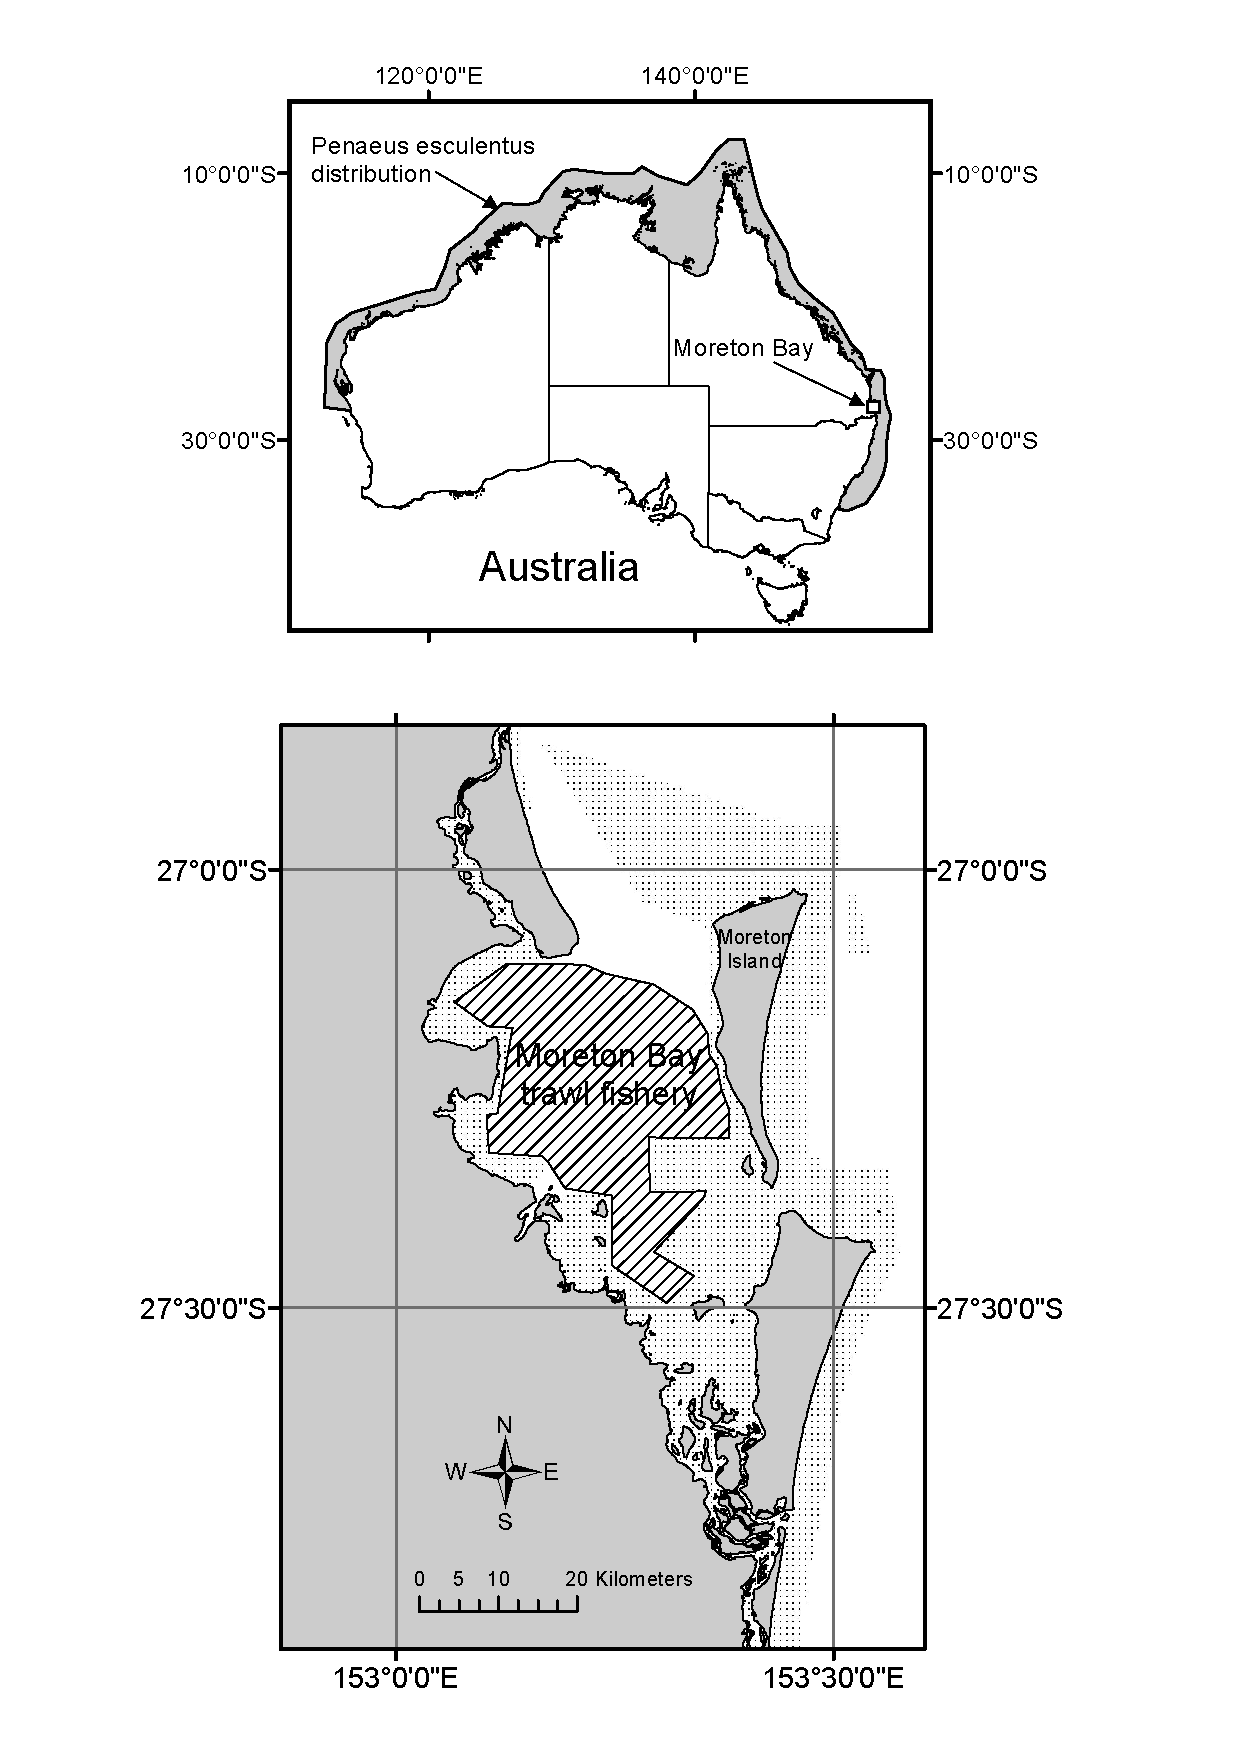
\includegraphics[scale=0.5, angle = 0]{MoretonBaytrawlfisheryandtigerprawndistribution3.ps}
       \caption{Top map: the spatial distribution of the brown tiger prawn ({\it Penaeus esculentus}) in Australia (from \cite{Grey83r}) with the location of Moreton Bay indicated by a black square. Bottom map: the location of trawling ground in Moreton Bay (greyed area) covering an ar
ea of about 800 km$^{2}$.}
       \label{fig:Map}
     \end{center}
  \end{figure}

%%%%%% Diagram of a MDP
\begin{figure}[!ht]
\begin{center}
%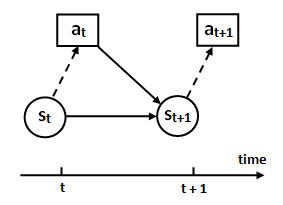
\includegraphics[width=0.2\textwidth,natwidth=300,natheight=100]{mdp.PNG}
\includegraphics{mdp.eps}
\end{center}
\caption[Decision diagram of a Markov Decision Process]{Decision diagram of a Markov Decision Process. Full arrows show relations of dependence, e.g. the value of $s_{t+1}$ (or $s'$) depends on $s_t$ (or $s$) through the probability $p$. Dashed arrows illustrate what factors the agent bases their decision upon; here, the best action is based on the current state only (Markov property).}
\label{fig:mdp}
\end{figure}

%%%%%% Beverton and Holt stock recruitment relationship
\begin{figure}[!ht]
  \begin{center}
        \includegraphics[scale=0.5,angle=-90]{BevertonAndHoltSRR-NaturalScale-WithCategories.eps}
    \caption{Beverton and Holt stock recruitment relationship fitted to the data. The recruitment categories used in the MDP are delimited with horizontal grey lines.}
    \label{fig:BevertonAndHoltSRR-NaturalScale-WithCategories}
  \end{center}
\end{figure}

%%%%%% Optimal catch using constant effort through time
\begin{figure}[!ht]
  \begin{center}
        \includegraphics[scale=0.6,angle=-90]{ProjectedCatchvsEffort.eps}
    \caption{Estimation of optimal yield, Maximum Average Yield (MAY), using constant effort of 20.500 boat-days per year through time.}
    \label{fig:ProjectedCatchvsEffort}
  \end{center}
\end{figure}


%%%%%% Pattern of fishing effort targeted at tiger prawn
\begin{figure}[!ht]
  \begin{center}
        \includegraphics[scale=0.5,angle=-90]{EffortPattern.eps}
    \caption{Average weekly pattern of fishing effort targeted at tiger prawn observed between 2006 and 2010.}
    \label{fig:EffortPattern}
  \end{center}
\end{figure}


%% Transition matrices
\begin{figure}[!ht]
  \begin{center}
        \includegraphics[scale=0.6,angle=-90]{BubblePlotOfTransitionMatrix.eps}
    \caption{Representation of the transition matrices giving the probability of fishery to move from a given level of recruitment (low, medium or high) in year $t$ (y-axis) and to any recruitment category in year $t+1$ (x-axis) for a range of fishing pressure: no fishing (top left panel); 19,000--20,000 boat-days (top right) and 29,000--30,000 boat-days (bottom left).}
    \label{fig:BubblePlotOfTransitionMatrix}
  \end{center}
\end{figure}

%% MDP results sensitivity to discount factor
\begin{figure}[!ht]
  \begin{center}
        \includegraphics[scale=1,angle=-90]{SensitivityToDiscountFactor.eps}
    \caption{Sensitivity analysis of the MDP results to the value of the discount factor ($\gamma$) for prawn price fixed at \$12/kg. Each panel shows the optimal fishing effort (y-axis) to maximize profit according to recruitment level (x-axis) for a discount factor value at various costs of fishing ranging from \$0 to \$500 per boat-day (see legend). The horizontal dashed line indicates effort at MAY (${\rm E_{MAY}=19,500 boat-days}$). More details are given in supplemental material, Fig.~\ref{fig:SensitivityToDiscountFactorLONGVERSION}.}
    \label{fig:SensitivityToDiscountFactor}
  \end{center}
\end{figure}

    
%% Optimal strategy according to the MDP 
%\begin{figure}[!ht]
%  \begin{center}
%        \includegraphics[scale=0.6,angle=-90]{MDPonProfit_finalVersion.eps}
%     \caption{Optimal fishing effort (y-axis) in response to the state of the fishery (x-axis) given a prawn price of 12\$/kg and fishing costs varying from 0 to 500\$ per boat-day. The horizontal dotted line indicates the effort required to achieve Maximum Average Yield (${\rm E_{MAY}}$)).}
%    \label{fig:MDPonProfit}
%  \end{center}
%\end{figure}

%% Compare MDP results with observations
\begin{figure}[!ht]
   \subfigure[]{ % FROM THE SUBFIGURE PACKAGE
    \label{fig:PlotEffortAgainstRecruitment}
    \begin{minipage}[b]{0.5\textwidth}
          \includegraphics[scale=0.45, angle = -90]{PlotEffortAgainstRecruitment.eps}
   \end{minipage}
}
 \subfigure[]{ % FROM THE SUBFIGURE PACKAGE
    \label{fig:MDPonProfit-OverlayedWithObs}
    \begin{minipage}[b]{0.5\textwidth}
          \includegraphics[scale=0.45, angle = -90]{MDPonProfit-OverlayedWithObs.eps}
   \end{minipage}
}
%% Plot MDP results on a yield (y-axis) versus recruitment (x-axis) plot as presented by Hilborn & Walters (1992) p.455
   \subfigure[]{ % FROM THE SUBFIGURE PACKAGE
    \label{fig:MDPonProfit-RecCatAgainstCatch-OverlayedWithObs}
    \begin{minipage}[b]{0.5\textwidth}
          \includegraphics[scale=0.45, angle = -90]{MDPonProfit-PlottedAgainstCatchOverlayedWithObs.eps}
          \label{MDPonProfit-RecCatAgainstCatch-OverlayedWithObs}
          \end{minipage}
          }
     \caption{Comparison of MDP optimal policies to observations: (a) observed relation between recruitment (x-axis) and effort (y-axis) with regression line overlayed (b) optimal strategies for $\gamma=0.8$ overlayed with observed effort (grey circles) and recruitment binned into the discrete categories used for the MDP (c) Average yield from each optimal strategy overlayed with observed yield as a function of recruitment category in each year. The horizontal dotted line indicates the Maximum Average Yield (MAY) or $\rm{E_{MAY}}$.}
    \label{}
  \end{figure}

%% Effect of varying prawn prices on MDP outcomes
\begin{figure}[!ht]
  \begin{center}
    \includegraphics[scale=1, angle=-90]{SensitivityToPrawnPrice.eps}
    \caption{Effect of varying prawn prices on optimal fishing policies. Each panel shows the optimal fishing effort (y-axis) to maximize profit according to recruitment level (x-axis) for various prawn prices ($P$) varying from \$12 to \$100 per kg for various costs of fishing ranging from 0 to \$500 per boat-day (see legend).}
    \label{fig:SensitivityToPrawnPrice}
  \end{center}
\end{figure}


%% Simulate states, actions and rewards of various strategies
\begin{figure}[!ht]
   \subfigure[]{ % FROM THE SUBFIGURE PACKAGE
    \label{fig:CompareVariousStrategies-1Simulation-TimeseriesOfStates}
    \begin{minipage}[b]{0.5\textwidth}
          \includegraphics[scale=0.25, angle = -90]{CompareVariousStrategies-1Simulation-TimeseriesStatesAndActionsOptimalAndRandomEffort.eps}
   \end{minipage}
}
 \subfigure[]{ % FROM THE SUBFIGURE PACKAGE
    \label{fig:CompareVariousStrategies-1Simulation-TimeseriesOfActions}
    \begin{minipage}[b]{0.5\textwidth}
          \includegraphics[scale=0.25, angle = -90]{CompareVariousStrategies-1Simulation-TimeseriesStatesAndActionsCteEffortLowAndMay.eps}
   \end{minipage}
}
   \subfigure[]{ % FROM THE SUBFIGURE PACKAGE
    \label{fig:CompareVariousStrategies-1Simulation-CumulativeReward}
    \begin{minipage}[b]{0.5\textwidth}
          \includegraphics[scale=0.25, angle = -90]{CompareVariousStrategies-1Simulation-AverageYearlyReward.eps}
          \end{minipage}
          }
    \subfigure[]{ % FROM THE SUBFIGURE PACKAGE
    \label{fig:CompareVariousStrategies-repeat1000times}
    \begin{minipage}[b]{0.5\textwidth}
          \includegraphics[scale=0.25, angle = -90]{CompareVariousStrategies-repeat1000times.eps}
          \end{minipage}
          }
         
     \caption{Simulations comparing the performance of 4 harvest strategies: (1) the optimal harvest strategy; (2) a random fishing strategy; (3) a constant low effort fishing strategy  and (4) a constant effort strategy at ${\rm{E_{MAY}}}$. These simulations were performed for a cost of fishing of \$200 per boat-day and a price of prawns of \$12 per kg. Panel (a) shows time series from a single simulation of tiger prawn recruitment (states) and effort category (actions) according to the optimal and the random effort strategy over a 50 years period. Panel (b) shows the same variables for constant low and constant $E_{\rm MAY}$ strategy. Panel (c) shows the average yearly profit made by each strategy. Panel (d) summarizes the average yearly profit according to each strategy for 1000 simulations over a 50 year period.}
    \label{fig:simulations}
  \end{figure}



%% 
%\begin{figure}[!ht]
%  \begin{center}
%    \includegraphics[scale=0.5,angle=-90]{EffortSurface.eps}
%    \caption{Isoclines of average action category as a function of prawn price per kilo (y-axis) and cost of 1 fishing boat-day (x-axis).}
%    \label{fig:EffortSurface}
%  \end{center}
%\end{figure}


%\clearpage
%\newpage
%\section*{Tables}
%% latex table generated in R 3.3.3 by xtable 1.8-2 package
% Tue Mar 28 14:10:15 2017
\begin{table}[ht]
\centering
\begin{tabular}{rrrrrrrrrr}
  \hline
 & 8 & 10 & 12 & 14 & 16 & 18 & 20 & 22 & 24 \\ 
  \hline
100 & 5.4 & 9.2 & 13.3 & 17.1 & 21.7 & 26.9 & 31.8 & 36.6 & 41.5 \\ 
  150 & 2.6 & 5.2 & 8.1 & 11.8 & 15.8 & 19.9 & 24.1 & 27.8 & 32.6 \\ 
  200 & 1.1 & 2.7 & 5.0 & 7.8 & 10.8 & 14.4 & 18.4 & 22.4 & 26.5 \\ 
  250 & 0.4 & 1.3 & 2.9 & 5.1 & 7.7 & 10.5 & 13.5 & 17.1 & 21.0 \\ 
  300 & 0.1 & 0.5 & 1.6 & 3.2 & 5.2 & 7.5 & 10.4 & 13.1 & 16.3 \\ 
  350 & 0.0 & 0.2 & 0.7 & 1.9 & 3.4 & 5.2 & 7.6 & 10.3 & 13.0 \\ 
  400 & 0.0 & 0.0 & 0.4 & 0.9 & 2.1 & 3.7 & 5.3 & 7.7 & 10.0 \\ 
  450 & 0.0 & 0.0 & 0.1 & 0.6 & 1.0 & 2.4 & 3.9 & 5.6 & 7.7 \\ 
  500 & 0.0 & 0.0 & 0.0 & 0.3 & 0.7 & 1.2 & 2.7 & 4.1 & 5.8 \\ 
   \hline
\end{tabular}
\caption{Total profit, in millions of dollar, as a function of the prices of prawns per kilos (columns) and the cost of 1 boat-day fishing (in rows).} 
\label{tab:AverageValueAsFctPricesAndCosts}
\end{table}


%%%%%%%%%% Merge with supplemental materials %%%%%%%%%%
\clearpage
\begin{center}
\textbf{\large Supplemental Materials: Optimal Harvest Strategies according to a Markov Decision Process applied to a delay-difference model: insights from the tiger prawn fishery in Moreton Bay (Australia)}
\end{center}

%%%%%%%%%% Merge with supplemental materials %%%%%%%%%%
%%%%%%%%%% Prefix a "S" to all equations, figures, tables and reset the counter %%%%%%%%%%
\setcounter{section}{0}
\setcounter{equation}{0}
\setcounter{figure}{0}
\setcounter{table}{0}
\setcounter{page}{1}
\makeatletter
\renewcommand{\thesection}{S\arabic{section}}
\renewcommand{\theequation}{S\arabic{equation}}
\renewcommand{\thefigure}{S\arabic{figure}}
\renewcommand{\bibnumfmt}[1]{[S#1]}
\renewcommand{\citenumfont}[1]{S#1}
%%%%%%%%%% Prefix a "S" to all equations, figures, tables and reset the counter %%%%%%%%%%

%% Policy iteration algorithm
\section{Policy iteration algorithm}
\label{SuppSection-PolicyIterationAlgo}

Policy iteration unfolds as follows: starting from any initial policy $\pi_0$, the best current policy $\pi$ is evaluated (step 1) and improved (step 2) repeatedly until it is optimal ($\pi^*$).  \\

1) The evaluation consists of calculating a value $V_\pi(s)$ for each state $s \in S$. This value corresponds to the sum of future rewards one can expect, starting from the state $s$ when implementing the policy $\pi$. The value function captures the desirability of the different states, and will help select the optimal actions. Formally,

\begin{equation}
V_\pi(s) = \mathbb{E}[\sum\limits_{t=0}^\infty \gamma^t r(s_t,\pi(s_t))|s_0=s]
\end{equation}

The following recursive formula holds: 

\begin{equation}
V_\pi(s) = r(s,\pi(s)) + \gamma \sum_{s' \in S} P(s'|s,\pi(s)) V_\pi(s')
\end{equation}

This can be calculated recursively (applying this formula until convergence of $V_\pi$) or by solving the following linear system, since the value function can be rewritten: 

\begin{equation}
V_\pi = r_\pi + \gamma P_\pi V_\pi
\end{equation}
with $r_\pi$ and $P_\pi$ the reward and transition matrix associated with the policy $\pi$. Denoting by $I$ the identity matrix, this implies

\begin{equation}
V_\pi = (I-\gamma P_\pi)^{-1}r_\pi  \label{eq:evaluation}
\end{equation}

Note that $I-\gamma P_\pi$ is always invertible when $\gamma<1$ because $P_\pi$ is a transition matrix. \\

2) Once the value $V_\pi$ has been evaluated, we can improve the policy $\pi$ by selecting the best actions (Bellman's equation \citep{bellman_dynamic_1957, puterman_markov_1994}): 

\begin{equation} \label{eq:improvement}
\pi(s) = \argmax_{a \in A} [r(s,a)+ \gamma \sum_{s' \in S} P(s'|s,a)V_\pi(s')]
\end{equation}

Equations \ref{eq:evaluation} and \ref{eq:improvement} are computed several times until the policy $\pi$ converges to the optimal policy $\pi^*$ using the MDPtoolbox package in R \citep{MDPtoolbox}. The sequence of $V_\pi$ is monotonic, so convergence is guaranteed \citep{sigaud_markov_2010}. The outputs of policy iteration are the optimal policy $\pi^*$ and the optimal value $V_\pi^*$. \\

%%%%%%%%%%%%%%%%%%%%%%%%%%%%%%%%%%%%%%%%%%%%%%%%%%%
\clearpage
\newpage
\section*{Figures}


%% MDP results sensitivity to discount factor
\begin{figure}[!ht]
  \begin{center}
        \includegraphics[scale=0.85,angle=-90]{SensitivityToDiscountFactorLONGVERSION.eps}
    \caption{Sensitivity analysis of the MDP results to the value of the discount factor ($\gamma$). Each panel shows the optimal fishing effort (y-axis) to maximize profit according to recruitment level (x-axis) for a discount factor value at various costs of fishing ranging from \$0 to \$500 per boat-day (see legend). The horizontal dashed line indicates effort at MAY (${\rm E_{MAY}}$).}
    \label{fig:SensitivityToDiscountFactorLONGVERSION}
  \end{center}
\end{figure}

\end{document}









